\newpage
\section{Speech Signal Processing}

\subsection{Analog-to-Digital Conversion}
Voices in real life are analog signals, hence before conducting digital signal processing techniques, analog-to-digital conversions are required.\\

Given a continuous-time signal $s(t)$, we define the \textit{sampled signal} by
\begin{equation}
s[n] = s(nT_s) = s(\frac{n}{F_s})
\end{equation}
where $T_s$ is the sampling interval and $F_s$ is the sampling rate.\\

$T_s$ should be carefully chosen in order to avoid distortion caused by aliasing. Telephony since the 1950s limits the information bandwidth to 300-3400 Hz \cite{EVW-report}. However, in normal conversational speech, the frequency content is mainly between 0-8000 Hz \cite{uysal2005bandwidth}. According to Nyquist-Shannon sampling theorem, we set the folding frequency $\frac{F_s}{2}$ = 8000 Hz, i.e. $F_s$ = 16 kHz.

%--------------------------------------------
%--------------------------------------------

\subsection{Pre-emphasis}

The speech production system inherently attenuates speech signal by a negative spectral slope per decade. In addition, human hearing is more sensitive to frequency band above 1 kHz \cite{picone1993signal}. However, as is depicted in Fig. \ref{zero_fft}, frequency components below 1 kHz predominantly comprise the spectrum. Hence, it is advantageous to employ a high-pass filter to amplify the high frequency range.

\begin{figure}[H]
\centering
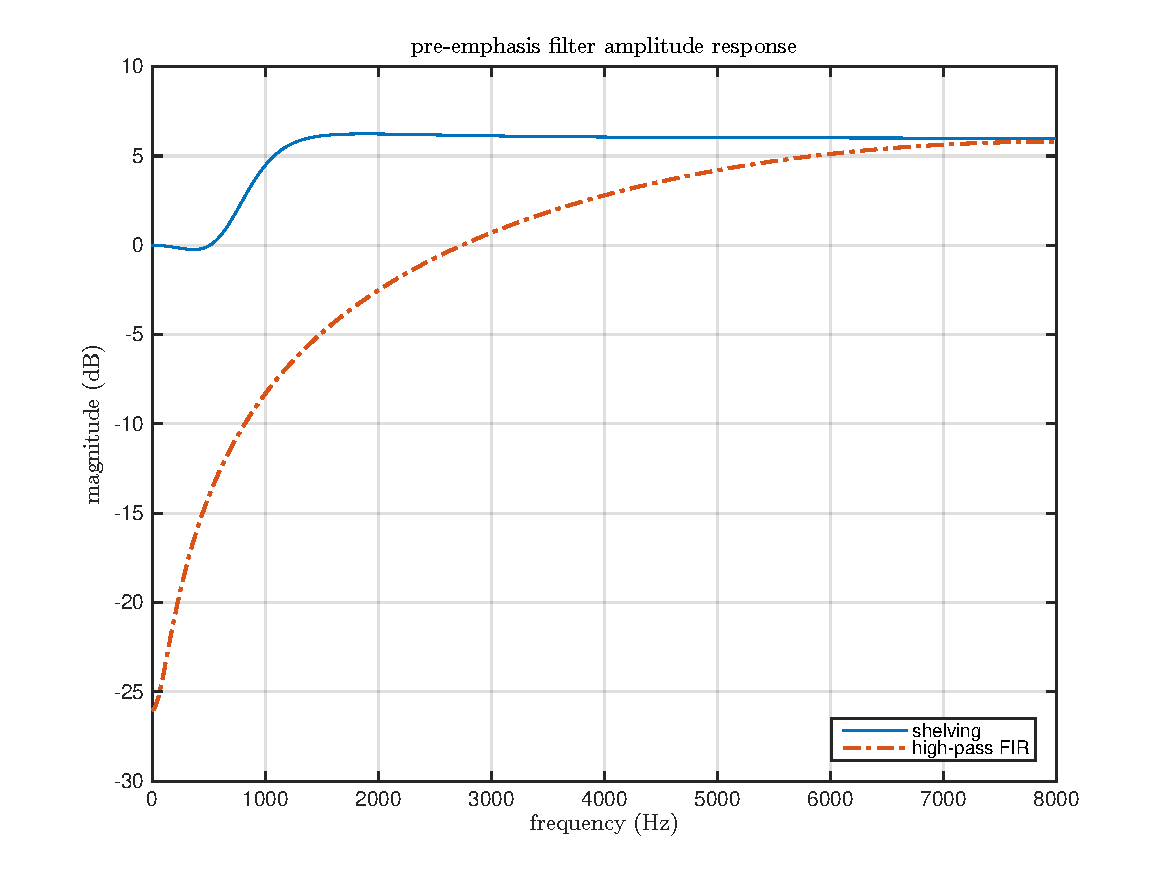
\includegraphics[width=6in]{ang/pre_emphasis_filter}
\caption{Pre-emphasis Filters Comparison}
\label{pre_emphasis_filter}
\end{figure}

\begin{equation}
\label{high-pass-filter}
y[n] = x[n] - \alpha x[n-1]
\end{equation}

A 1st-order FIR filter represented by (\ref{high-pass-filter}) is widely implemented, including the previous group where $\alpha = 0.95$ \cite{EVW-report}. The merits of this FIR filter include simplicity and efficiency. However, Fig. \ref{pre_emphasis_filter} (red dash-dot line) shows that frequencies below 500 Hz are severely suppressed even though frequencies above 3 kHz are successfully amplified. Considering the potential interference caused by high-frequency noise, attenuating low frequencies too much will result in the decline of signal-to-noise ratio (SNR).

\begin{equation}
\label{shelving-filter}
y[n] = \frac{1}{a_0} \big( b_0 x[n] + b_1 x[n-1] + b_2 x[n-3] \big) - (a_1 y[n-1] + a_2 y[n-2])
\end{equation}

Suggested by Professor Erik \textsc{Weyer}, we try to devise a shelving filter represented by (\ref{shelving-filter}) to pre-emphasize the speech signal. By trial and error, we eventually manage to obtain a appropriate filter that amplifies high frequency without attenuating low frequencies (shown in Fig. \ref{pre_emphasis_filter} by blue solid line), where

\begin{align*}
&\begin{cases}
a_0 = 0.25\\
a_1 = -0.380949\\
a_2 = 0.162336
\end{cases}
&\begin{cases}
b_0 = 0.465464\\
b_1 = -0.775712\\
b_2 = 0.341636
\end{cases}
\end{align*}

\begin{figure}[H]
\centering
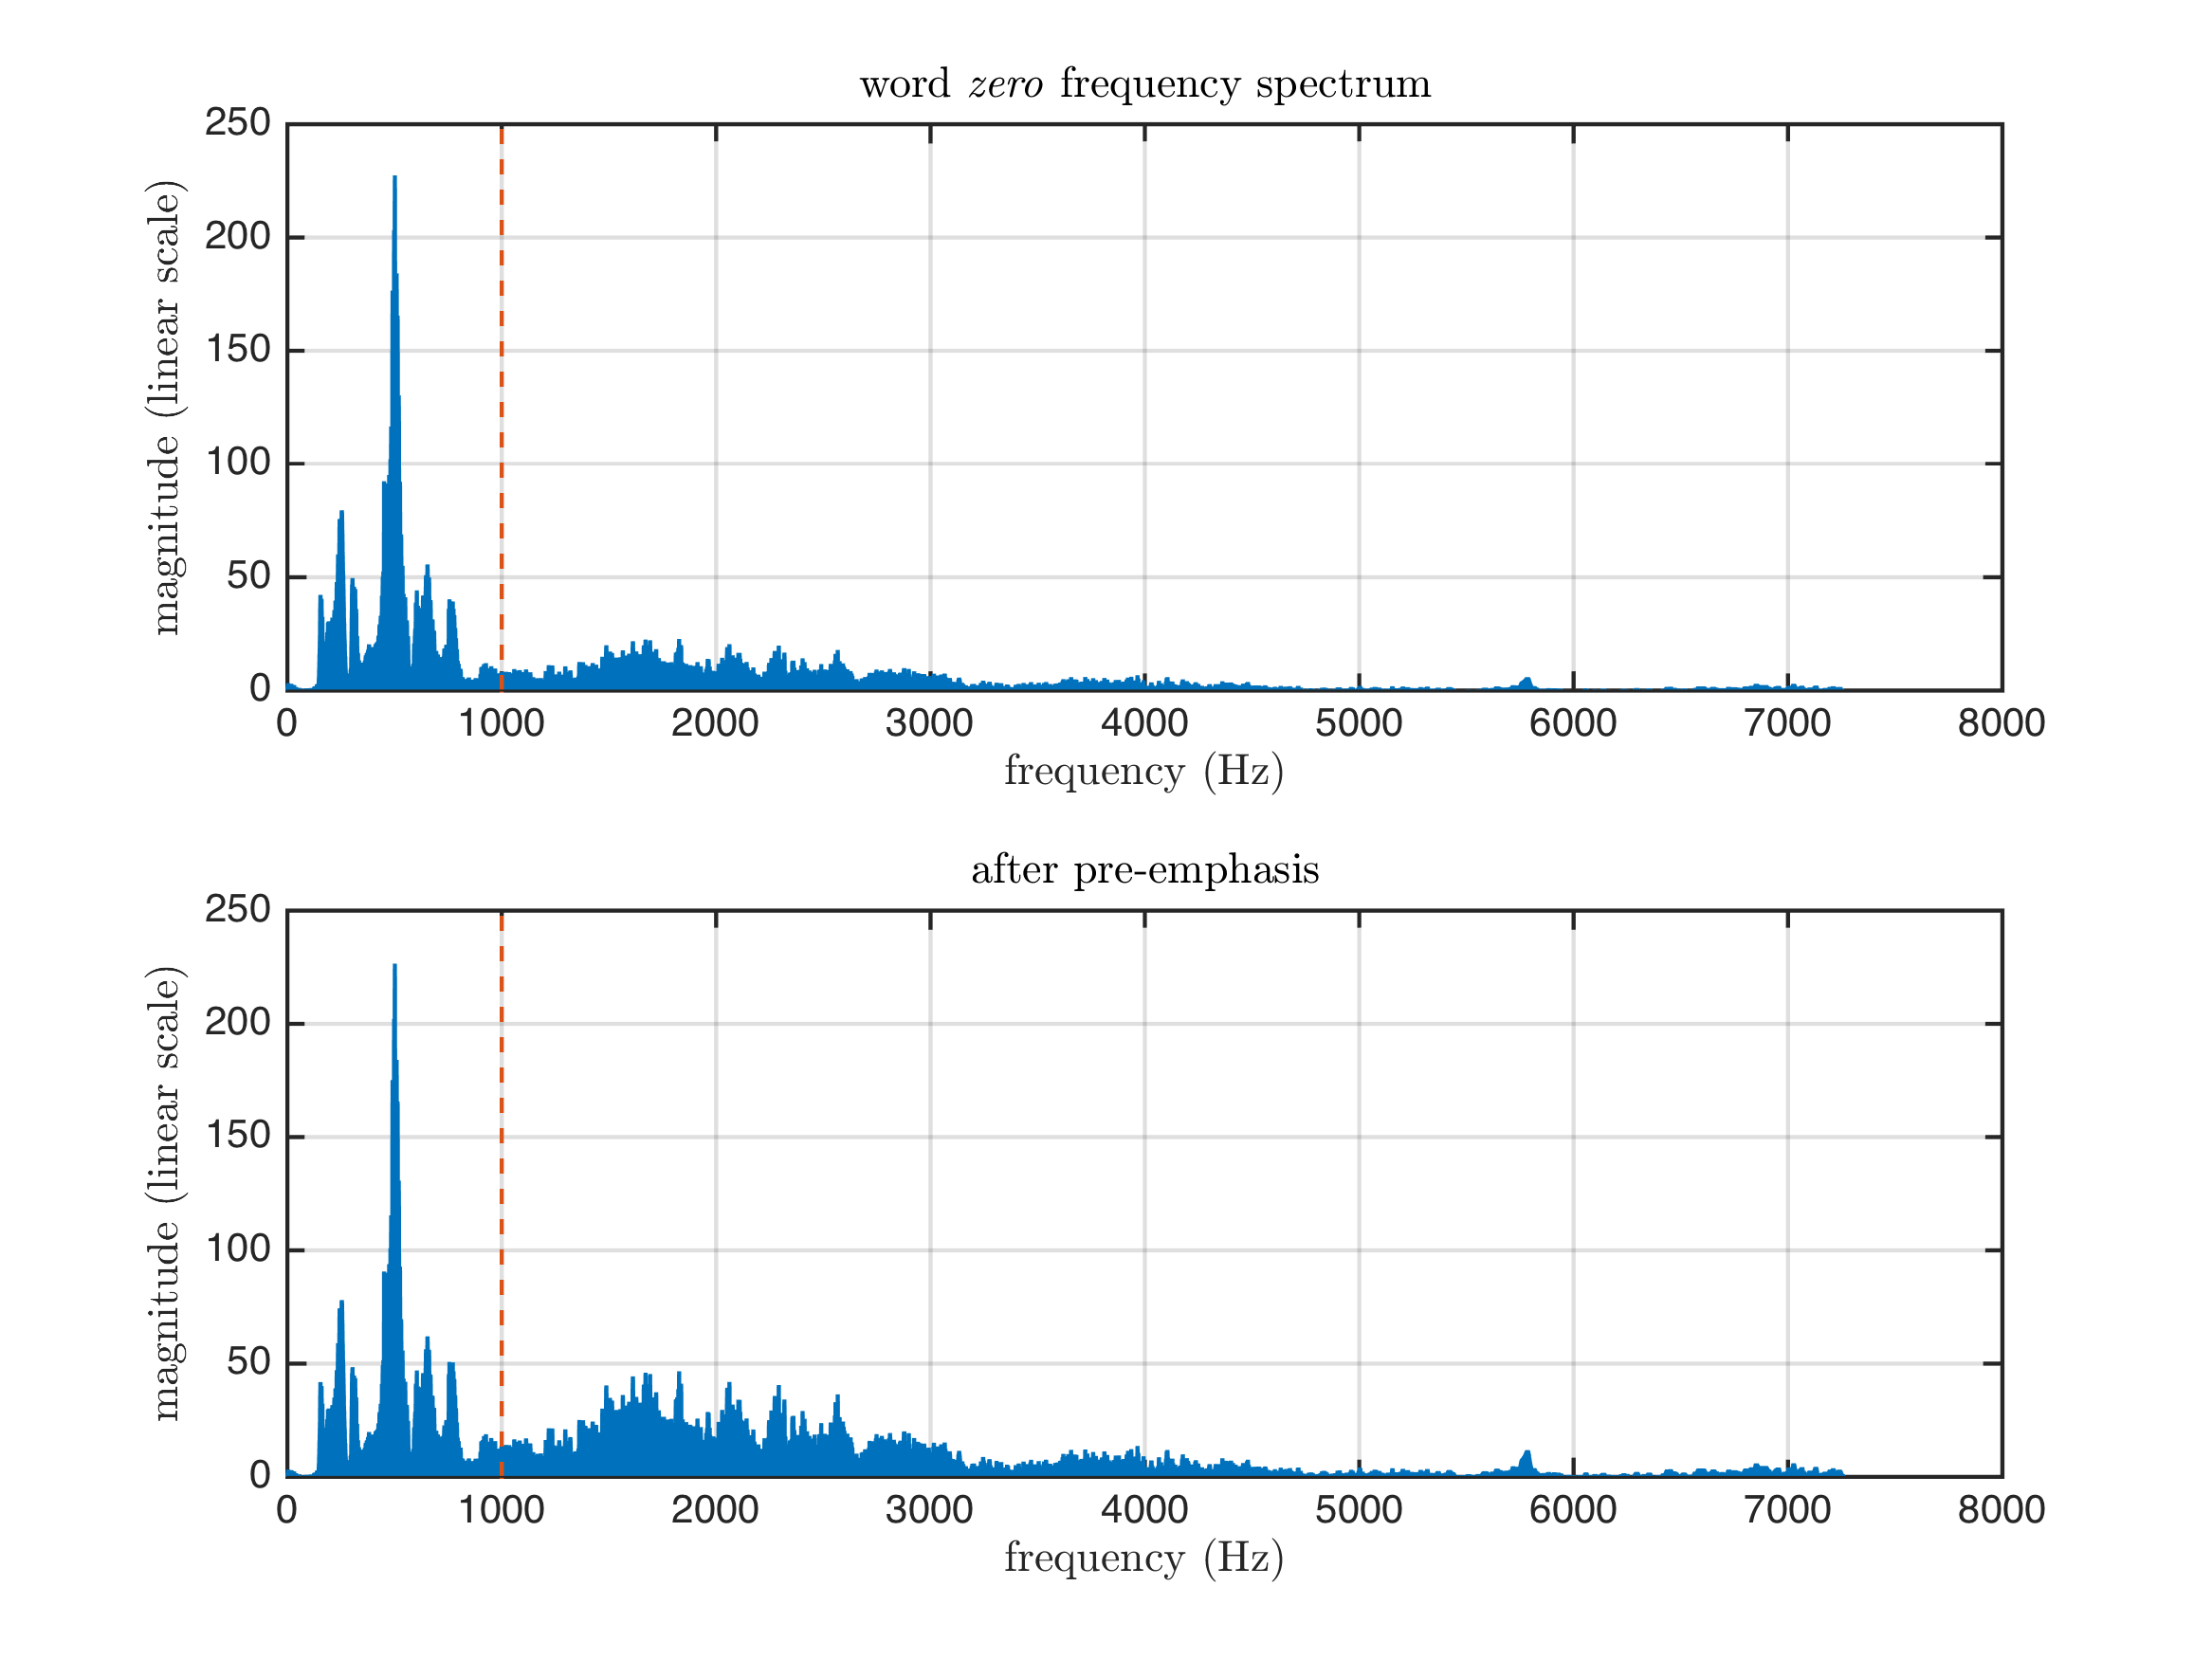
\includegraphics[width=\textwidth]{ang/zero_fft}
\caption{Word `zero' Spectral Analysis}
\label{zero_fft}
\end{figure}

%--------------------------------------------
%--------------------------------------------

\subsection{Framing \& Windowing}

%--------------------------------------------
%--------------------------------------------

\subsection{Threshold}

%--------------------------------------------
%--------------------------------------------

\subsection{Mel Filter Bank Processing}

\subsubsection{Power Spectrum}

%--------------------------------------------

\subsubsection{Bank Filtering}

\begin{figure}[H]
\centering
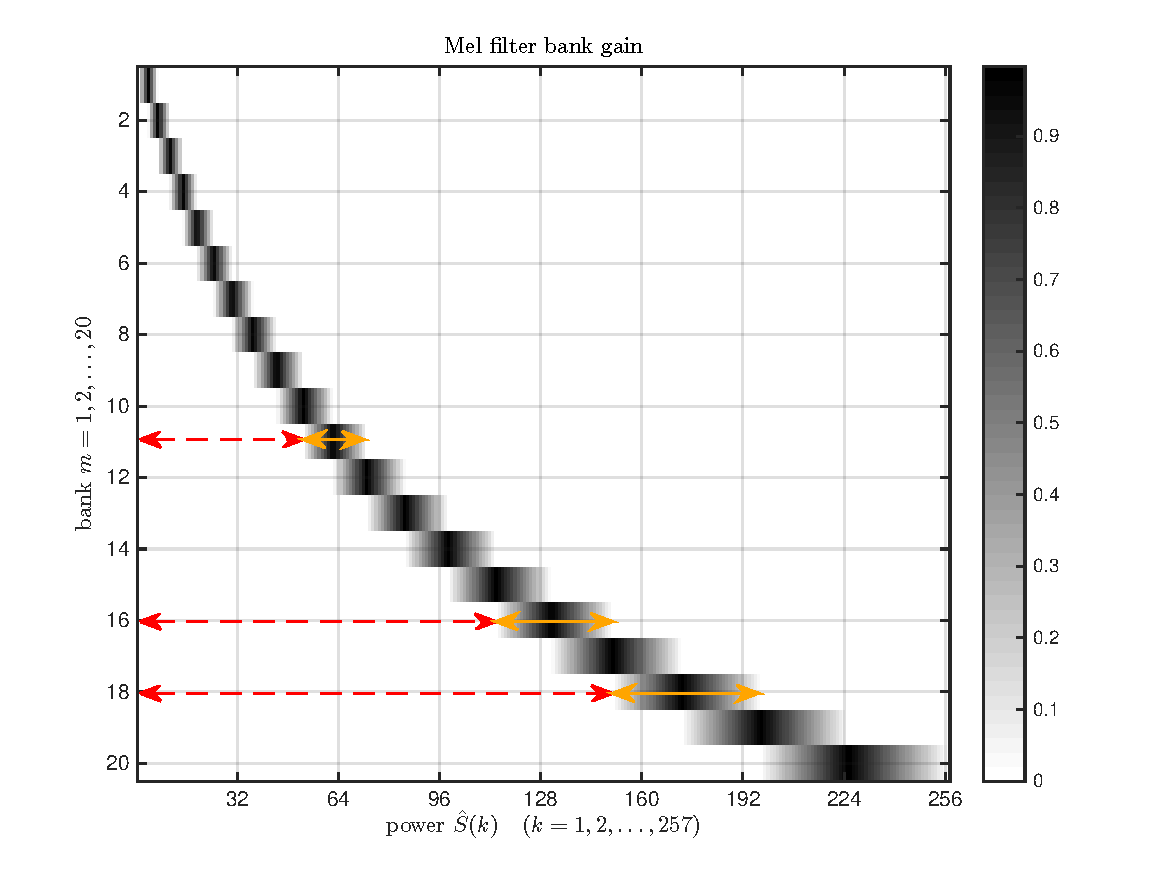
\includegraphics[width=6in]{ang/mel_filter_bank_gain}
\caption{Mel Filter Bank Gain}
\end{figure}

\begin{figure}[H]
\centering
\includegraphics[width=6in]{ang/mel_bank_9}
\caption{Bank Filtering Demonstration}
\end{figure}

%--------------------------------------------

\subsubsection{Log Scaling}

%--------------------------------------------

\subsubsection{Discrete Cosine Transform}
